

\chapter{Backgroud}

\section{Introductory Remarks}

Bitcoin or any other digital form of money by nature is an interesting idea for the 21st century, but how practical and useful these would be to the people living in this era is what would make a difference. 
In this research, we tried to have a real world view of the implications that Bitcoin usage could have and also evaluated the existing approaches to holding, using and accepting Bitcoin as a digital form of money.


%\subsection{Digital Cash}
%The concept of digital cash was introduced by David Chaum in 1983 ~\cite{chaum1983blind}, he continued the idea and founded a company named DigiCash\footnote{\url{https://en.wikipedia.org/wiki/DigiCash}} as a digital cash company but filed for bankruptcy in 1998. In the same year, Paypal\footnote{\url{http://paypal.com}} emerged and other systems such as E-gold \footnote{\url{https://en.wikipedia.org/wiki/E-gold}} followed but due to criminal usage of E-gold they got shut down in 2005 by United States Federal. In 2008, Bitcoin was introduced and solved most of the problems of all the digital cashes before it which marked the start of digital currencies.



\section{Bitcoin}
Bitcoin is a cryptographic currency deployed in 2009~\cite{Nak08}, which has reached a level of adoption unrealized by decades of previously proposed digital currencies (from 1982~\cite{Cha82} onward). Unlike many previous proposals, Bitcoin does not distribute digital monetary units to users. Instead, a public ledger maintains a list of every transaction\footnote{Technically, a transaction specifies a short script that encodes how the balance can be claimed as the input to some future transaction.} made by all Bitcoin users since the creation of the currency. A \textit{transaction} in its simplest form describes the movement of some balance of the Bitcoin currency (XBT or BTC) from one or more accounts (called input addresses) into one or more accounts (called output addresses). Bitcoin addresses are indexed by the fingerprint of a public key from a digital signature scheme.\footnote{Elliptic Curve Digital Signature Algorithm (ECDSA)~\cite{ecdsa}.} They are not centrally allocated or registered in any way---the addresses become active when the first transaction moving money into them is added to the ledger. 

In Bitcoin, every standard transaction\footnote{From now on, the word transaction refers to a standard transaction unless otherwise specified} must be digitally signed using the private signing key associated with each input address in the transaction. In order to spend Bitcoin, users require access to the signing key of the account holding their Bitcoin. Thus users do not maintain any kind of units of currency; they maintain a set of keys that provide them signing authority over certain accounts recorded in the ledger. 

The ledger (known as the \emph{blockchain}) is maintained and updated by a decentralized network using a novel method to reach consensus that involves incentivizing nodes in the network with the ability to generate (known as mining) new Bitcoin and collect transaction fees. The details of the Bitcoin consensus model are not relevant to this thesis, but we note that clients in the network participate in the consensus model by downloading and cryptographically verifying the integrity of the blockchain. As of writing, the Bitcoin blockchain is roughly 30 GB in size.


Due to the large size of the Bitcoin blockchain, full download is infeasible for thin clients running on mobile devices, as well as some desktop clients. These clients connect to a semi-trusted nodes and only request transactions relevant to keys in their wallet. This technique, known as Simplified Payment Verification (SPV), eliminates the need to download and verify the entire blockchain but, when implemented incorrectly, can create privacy risks~\cite{SPVbugs}. Also it has integrity risks, in the sense that it cannot forge transactions but could omit reports of relevant transactions.
%MOVED to chap0 backgroud
%Bitcoin is the first decentralized virtual currency and by far has adopted the most number of users ~\cite{Nak08}. it is based on cryptographic functions to remove the need of a central bank and regulates the generation of new units. 
%Bitcoin, as a protocol and as a currency, is a really vast subject that most would fall out of the scope of this thesis. We will try to cover Bitcoin as the currency and just the functionality of the protocol that is needed in order to hold and use Bitcoin as a currency.


%This introduction is not an introduction to Bitcoin, but the details of Bitcoin that are needed in this research.
In this section, we focus on introducing the essential constituents of Bitcoin that is needed in this research. Some details have been simplified to prevent going outside the scope of this thesis. Every aspect of Bitcoin that is missing from this introduction is explained through this thesis when the preliminary information of the usage is known to the reader.


\subsection{Bitcoin Address}
A Bitcoin address is a random string of 26-35 alphanumeric characters that starts with "1" or "3", that contains digits, uppercase and lowercase letters with the exception of "O", "I" (Uppercase i) , "l" (Lower case L) and the number 0 to prevent visual ambiguity. Bitcoin addresses are commonly shared via QR-Code as it is easier to read with QR-code mobile scanners and it is also implemented in almost all Bitcoin wallets (see figure ~\ref{fig:Bitcoinqr} that is a representation of the Bitcoin address 1shaYanre36PBhspFL9zG7nt6tfDhxQ4u). Bitcoin addresses are derived from the equivalent ECDSA public key that is explained later.

\begin{figure}
\centering
\includegraphics[scale=0.8]{fig/Bitcoinqr.png}
  \caption{QR-Code representing a Bitcoin address}
\label{fig:Bitcoinqr}
\end{figure}

\subsubsection{Public Key}
 In other words Bitcoin address is 160-bit hash of the public portion of the public and private ECDSA keypair. A public key is derived from the private key by some cryptographic functions (see Figure ~\ref{fig:pubkeytoaddr}). 

\begin{figure}
\centering
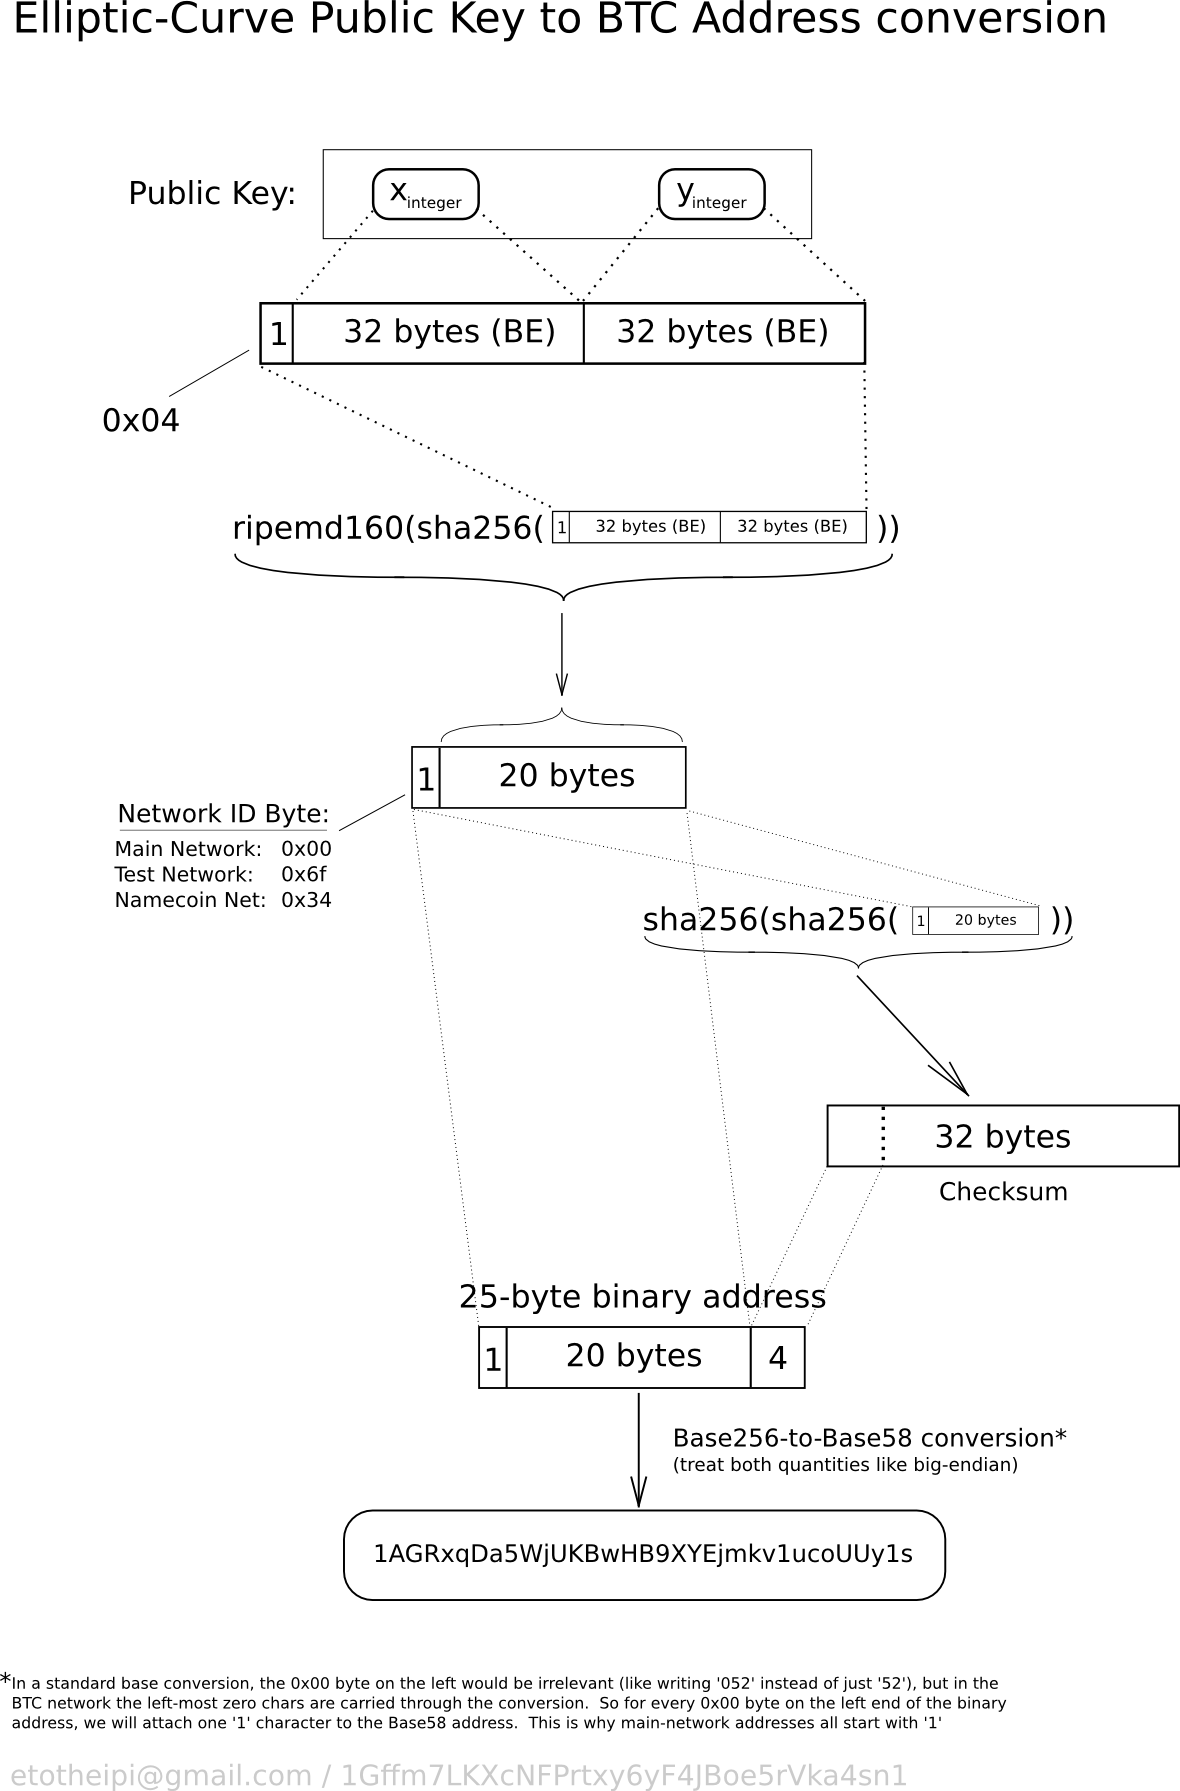
\includegraphics[width=\linewidth]{fig/PubKeyToAddr.png}
  \caption{ECDSA Public key to Bitcoin Address ~\cite{techaddress}}
\label{fig:pubkeytoaddr}
\end{figure}


\subsubsection{Private Key}
A private key can be any 256 bit number from 0x1 to 0xFFFF FFFF FFFF FFFF FFFF FFFF FFFF FFFE BAAE DCE6 AF48 A03B BFD2 5E8C D036 4140. Basically any number in this range would be valid as the input for secp256k1\footnote{Standards for Efficient Cryptography (SEC) \url{https://en.Bitcoin.it/wiki/Secp256k1}} ECDSA standard. This is the secret part of the Bitcoin address that should be kept secure and there are already different methods of securing the private key as discussed in Chapter 3. Anyone with the private key has the ability to sign a transaction and spend the Bitcoins that are signed with the relevant public key (or Bitcoin address). 
Same as the Bitcoin addresses and the public keys, private keys have a shorter format called wallet import format (wif) that is used commonly by most Bitcoin wallet clients. It contains error checking bits and also some information about the public key associated to the private key. An example of a private key in wif format would be 5Kb8kLf9zgWQnogidDA76MzPL6TsZZY36hWXMssSzNydYXYB9KF which would result in 1CC3X2gu58d6wXUWMffpuzN9JAfTUWu4Kj as the associated Bitcoin address.

To better understand how Bitcoin address is derived from the private key see Figure  ~\ref{fig:pubkeytoaddr}.

\subsubsection{BIP32} \label{BIP32}
As Bitcoin creator, Satoshi Nakamoto ~\cite{Nak08} also points out, it's better to generate a new address for each transaction and receive the changes in a new change address (The concept of change addresses is explained more in chapter 3) to use the pseudonymity of Bitcoin. This brought a challenge to Bitcoin wallet client designs as keeping track of all the addresses in the wallet file, and also the ability to back up the private keys, could get complicated when there are hundreds of keys in the wallet (more in Chapter 3). \\
Bitcoin is an open source project, and to make improvements to the protocol there are Bitcoin Improvement Proposals (BIP) introduced by developers to be implemented in the core code. One important one is BIP32 also known as Hierarchical Deterministic Wallets or HD wallets ~\cite{bip32}. BIP32 introduces the ability to generate a tree of addresses from a single seed known as ''Master Seed''. A master node would be generated from the master seed and it is possible to branch it to multiple nodes shown as m/0, m/1, \dots, m/i , and then from each multiple addresses could be derived such as m/0/1, m/0/2, \etc. Each of these derivation has a path in the tree that is called ''BIP32 Path'' and is shown as ''m/0/1'' for second branch of the first branch of master seed m. Commonly the first branch would be used on different accounts and the second depth of nodes on the tree would be used as the addresses of each account. BIP32 simplifies the backing up process as there is just a seed to be backed up and it's easier to keep track of the addresses. BIP32 also allows a simple terminal that does not contain the private keys to generate new Bitcoin addresses (for use in point of sale terminals). A visualization of how BIP32 is design can be seen in figure ~\ref{fig:bip32}.

\begin{figure}
\centering
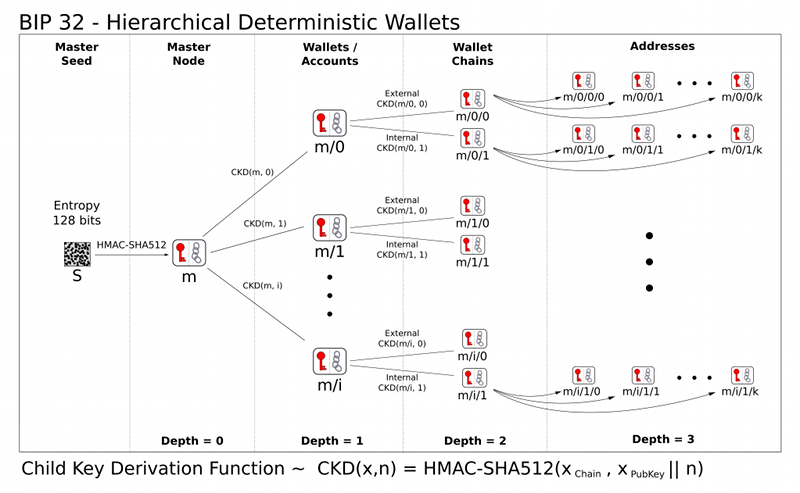
\includegraphics[width=\linewidth]{fig/bip32derivation.png}
  \caption{BIP32 - Hierarchical Deterministic Wallets ~\cite{bip32proposal}}
\label{fig:bip32}
\end{figure}


\subsection{Bitcoin Wallet}
This term has been conflated in Bitcoin sphere as both the file that contains the private keys and also the software client used to do mange Bitcoin transactions. This concept is more discussed in Chapter 3. For the sake of simplicity, we use the term Bitcoin wallet client as in the software used to sign Bitcoin transactions with the private key held in Bitcoin wallet file and manage the Bitcoin transactions.
The first and official Bitcoin wallet client is Bitcoin Core (Bitcoind as the daemon) that will be explained more on Chapter 3.


\subsection{Confirmation}
When a Bitcoin transaction broadcasts to the network, it should be included in a block by Bitcoin miners. Bitcoin miners are the computational devices which are using their hashing power (computational power) to verify each and every transaction within Bitcoin network and include them in a block. Each block would be added to the blockchain with a hash referencing its previous block and everyone in the network should form the consensus that the hash value for the block and the previous one is correct. As soon as the transaction is broadcasted it has 0-confirmation, that means it has not been added to any block, right after it gets included in a block it has 1 confirmation and this increases by each block that gets added to the blockchain.
It is possible for a miner\footnote{For the sake of simplicity of the language, in this thesis, we refer to the miners as ''He'', as in the operator of the mining devices. A miner is a computational device that could be operated by a single person or a group of people.} to fork the blockchain and start to mine blocks on his own fork, here is when the consensus model is important as the coins that were mined in his fork are invalid in the Bitcoin network and there is no reference in the main blockchain that those coins exists. The consensus model dictates that if a node sees two forks of the blockchain it should chose the longest chain. This check happens on every new block that is added to the blockchain and seen by the node.

\begin{figure}
\centering
\includegraphics[width=\linewidth]{fig/Bitcoinblocks.png}
  \caption{Bitcoin Blocks in the blockchain ~\cite{Nak08}}
\label{fig:Bitcoinblocks}
\end{figure}

This is important to understand that it is possible for a 0-confirmation transaction to stay unconfirmed for a while, depending on how much miner's fee is included in the transaction. Miner's tend to chose the transactions with a higher miner's fee to be included in the new block first, but this is not a universal fact since the miner is in control to chose which transactions should be included in the block he mined\footnote{This is why 51\% attack becomes noticable, as the miner that has 51\% of the hashing power would be in control to reject transactions specific to some addresses or whitelist some others to be included in new blocks. however he will not be able to forge transactions.}.

\subsection{Double Spend}
One of the major innovations of Bitcoin was to solve a problem known as double spending. For any digital data it is possible to duplicate the data and send it to two different entities, this could be a problem when this digital data has monetary value. Details of the solution would rely on a cryptographic description of how Bitcoin protocol works. However to put it in simple words, when spending some Bitcoins as an input to a transaction, the Bitcoin wallet should use the hash of those inputs that are already in the blockchain, when it broadcasts that transaction it will be stored on the memory of all the Bitcoin nodes as an unconfirmed transaction until it gets included in a block by a miner. Now it's possible to use the same input in another transaction and broadcast it to the network, mainly because that input was not spent in any blocks in the blockchain yet. Although only one of these transaction could be included in a new block and the other one would be invalid and erased from the memory. This makes it complicated for Bitcoin payment processors to accept 0-confirmation transactions as they could not be fully trusted. 



